\begin{figure}[h!]
  \centering   
    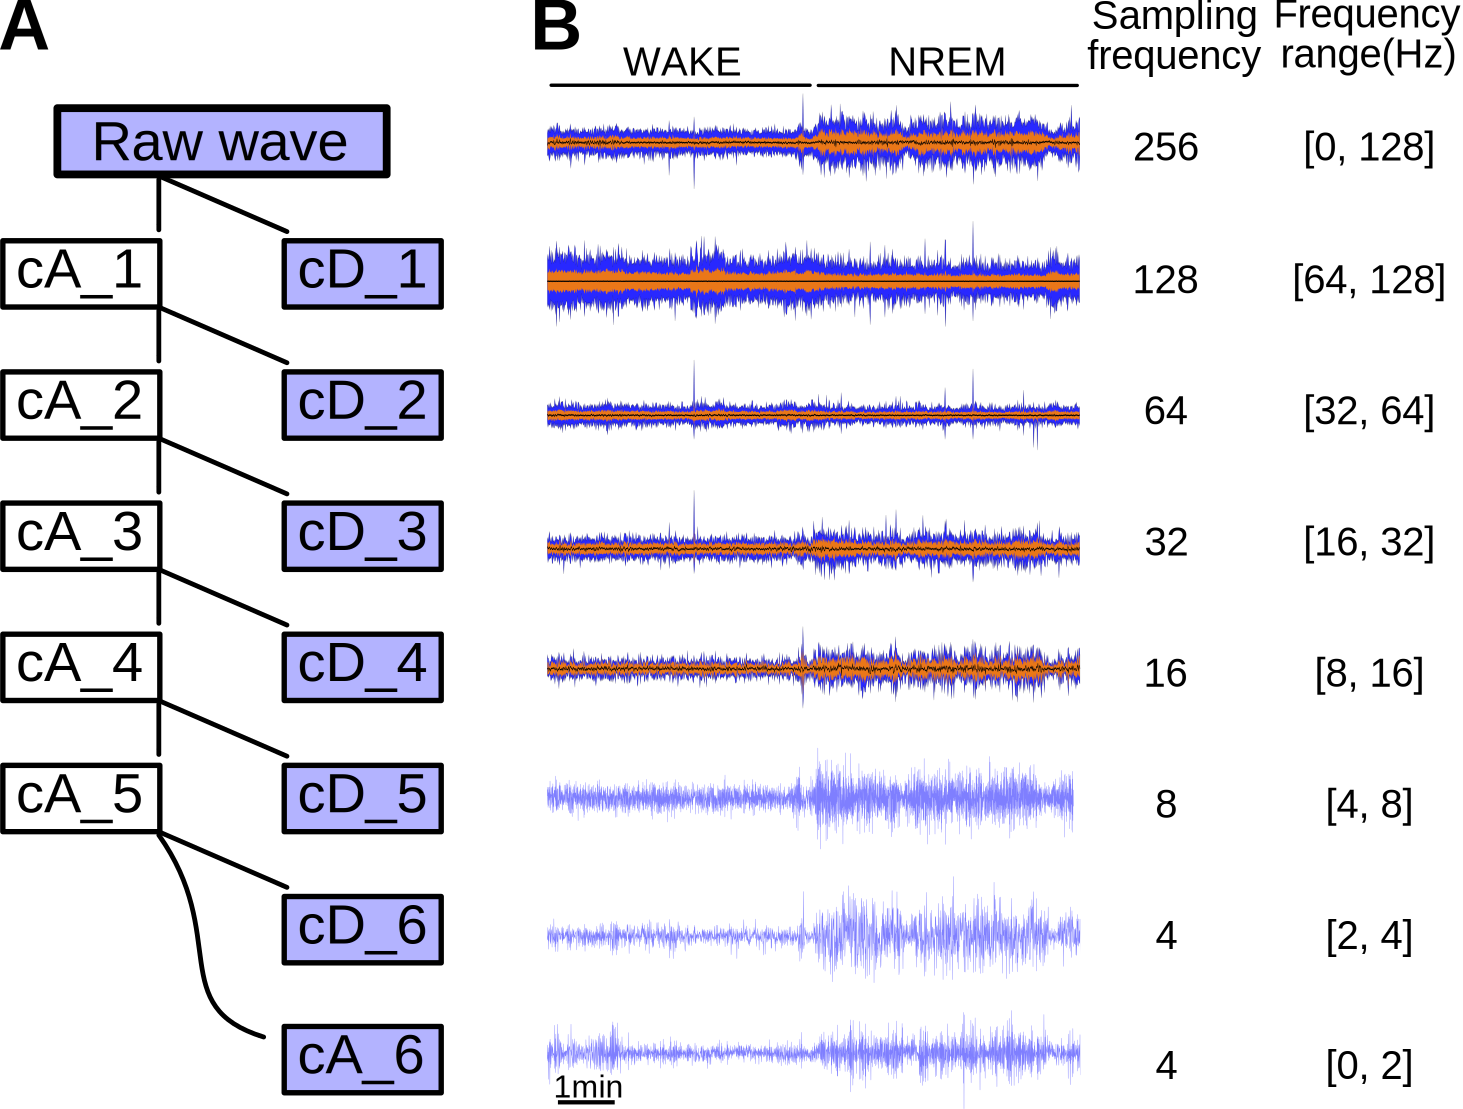
\includegraphics[width=0.95\textwidth]{figures/dwd.pdf}
  \caption{\ctit{Discrete wavelet decomposition.}
	\textbf{A}, Through discrete wavelet transform the initial signal is split into a pair of coefficients: $cA$ and $cD$, which capture the low ($[0, f_s/2]$), and high $[f_s/2, f_s]$ frequency information, respectively.
	Then, discrete wavelet transform is applied iteratively on subsequent $cA$ coefficients ($cA\_1, ..., cA\_n$), thus generating ($cD\_1, ..., cD\_n$).
	In this example, decomposition is performed up to the sixth level ($n=6$).
	\textbf{B}, 
	Ten minutes representing the \gls{eeg} of a transition between an awake episode and a slow wave sleep(NREM) are shown for the raw
	 wave and for each of the coefficients that are kept for feature extraction (blue rectangles in A).
	 The variation of amplitude in each coefficient corresponds to a concomitant variation of amplitude in its frequency range.
	 In this example, the general increase in power in the raw wave corresponds to an increase of power in the frequency bands below 32Hz, but with a decrease in power above 64Hz.
	%~ Later, each of the eight time series will be segmented into five second epochs, and features are computed for all epochs in the wavelet coefficients and the  raw signal.
	In this figure, the signals with $f_s > 8$ are too dense to render every point. 
	Instead, only local range(blue), inter-quantile range (orange) and median (black line) are represented.
  \label{fig:dwd}
  }
\end{figure}





